%!TEX root = ../main.tex

\chapter{Problema di classificazione}
\label{cha:problema_di_classificazione}

In un tipico problema di classificazione si hanno a disposizione un insieme di \textbf{caratteristiche} $f_1, f_2, \dots,f_n$ e un insieme di \textbf{classi} $c_1, c_2, \dots, c_m$: l'obiettivo consiste nel classificare degli \emph{oggetti} in base alle loro caratteristiche. Un oggetto può essere rappresentato in uno spazio $n$-dimensionale e pertanto è possibile trattare problemi di classificazione attraverso metodi geometrici.

Lo spazio multidimensionale è suddiviso in \textbf{regioni di decisione}, ovvero aree all'interno delle quali ricadono tutti gli oggetti di una classe. I \textbf{confini} di queste regioni sono determinate dalla rete attraverso il processo di addestramento.

Gli oggetti da classificare sono comunemente chiamati \textbf{pattern}. Una rete neurale impara a riconosce dei pattern a seguito di una \emph{fase di addestramento}, durante la quale alla rete vengono presentati un insieme di pattern di addestramento con l'indicazione della classe di appartenenza. Quando sarà presentato un nuovo pattern alla rete, appartenente ad una classeche questa ha precedentemente appreso, essa sarà in grado di classificarlo grazie alle informazioni estratte dai dati di addestramento.
\begin{figure}[h!]
	\centering
	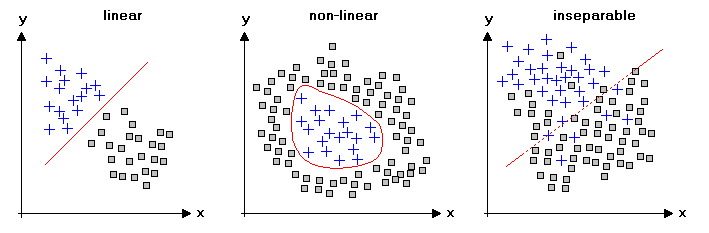
\includegraphics[width=\textwidth]{images/classify.png}
	\caption[Separabilità lineare nella classificazione.]{Rappresentazione geometrica di alcuni problemi di classificazione.}
\end{figure}

\noindent Quando si intende risolvere un problema di classificazione con una rete neurale, questa dovrà avere tante unità di input quante sono le caratteristiche degli oggetti e tanti neuroni di output quante sono le possibili classi.

\begin{figure}[h!]
	\centering
	\begin{tikzpicture}[->, node distance=\layersep]

		% Draw the input layer nodes
		\foreach \name / \y in {1,...,3}
		\node[input neuron, pin=left:$f_\y$] (I-\name) at (0,-\y) {};

		% Draw the output layer nodes
		\foreach \name / \y in {1,...,2}   
		\node[output neuron, pin={[pin edge={->}]right:$c_\y$}] (O-\name) at (\layersep, -\y cm - 0.5cm) {};

		% Connect every node in the input layer with every node in the output layer.
		\foreach \source in {1,...,3}
		\foreach \dest in {1,...,2}
		\path (I-\source) edge (O-\dest);
                
		% Annotate the layers
		\node[annot,above of=I-1, node distance=1cm] (il) {Input layer};
		\node[annot,right of=il] {Output layer};
	\end{tikzpicture}
	\caption[Esempio di percettrone.]{Rete feedforward ad uno strato usata per la classificazione.}
\end{figure}

\newpage

\section{Percettrone a singolo strato}
\label{sec:percettrone_a_singolo_strato}
La prima rete neurale utilizzata per risolvere problemi di classificazione è il \textbf{percettrone} di Rosenblatt (1958), un classificatore \textbf{binario} caratterizzato da un singolo strato con connessioni feedforward.

Il percettrone è un idea semplice ed elegante: imita il neurone umano ed è in grado di imparare da esempi che gli vengono presentati. Tuttavia, come dimostrato da M. Minsky e S. Papert (1969), ha una pesante limitazione: è in grado di risolvere solo problemi \textbf{linearmente separabili}, ovvero problemi in cui le regioni di decisione si possono separare con un iperpiano.

\begin{figure}[h!]
	\centering
	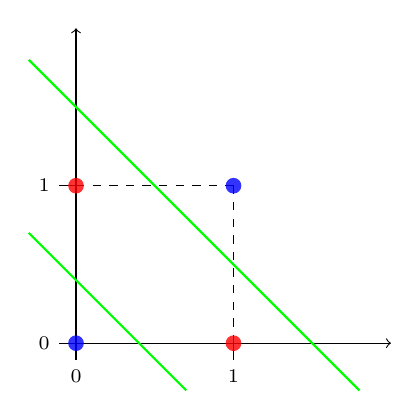
\begin{tikzpicture}[scale=2]
		
		% Axes
		\draw[->] (0,0) -- coordinate (x axis mid) (2,0);
		\draw[->] (0,0) -- coordinate (y axis mid) (0,2);
		
		% Ticks
		\foreach \x in {0,...,1}
		\draw (\x,1pt) -- (\x,-3pt)
		node[anchor=north] {\scriptsize\x};
		\foreach \y in {0,...,1}
		\draw (1pt,\y) -- (-3pt,\y)
		node[anchor=east] {\scriptsize\y};
		
		\draw[dashed] (1,0) -- (1,1);
		\draw[dashed] (0,1) -- (1,1);
		
		\draw[thick, color=green] (0.7,-0.3) -- (-0.3,0.7);
		\draw[thick, color=green] (-0.3,1.8) -- (1.8,-0.3);
		
		\node[fill=blue, circle, inner sep=2pt, opacity=0.8] at (0,0) {};
		\node[fill=red, circle, inner sep=2pt, opacity=0.8] at (0,1) {};
		\node[fill=red, circle, inner sep=2pt, opacity=0.8] at (1,0) {};
		\node[fill=blue, circle, inner sep=2pt, opacity=0.8] at (1,1) {};
		
		
	\end{tikzpicture}
	\caption{Non separabilità lineare dell'operatore XOR.}
\end{figure}

\noindent La convergenza del percettrone è garantita dal seguente teorema:
\begin{thm}[Teorema di convergenza del percettrone - N. J. Nilsson, 1965]
	Se il problema di classificazione è linearmente separabile allora la fase di apprendimento converge ad un'appropriata impostazione dei pesi in un numero finito di passi.
\end{thm}
Nella pratica non è dato sapere se un problema sia linearmente separabile o meno. La convergenza si può comunque ottenere aggiustando i parametri del percettrone come il numero di iterazioni o il fattore di apprendimento: in questo caso, tuttavia, la convergenza è artificiale.

\section{Percettrone a più strati}
\label{sec:percettrone_a_più_strati}

È possibile sopperire alle limitazioni dei percettroni a singolo strato aggiungendo strati di neuroni nascosti: il numero di strati, infatti, influenza la forma generale che possono assumere le regioni di decisione. Come si può osservare in figura \ref{fig:architetture}:
\begin{itemize}
	\item nelle reti a singolo strato si possono avere regioni di decisione separabili mediante un \textbf{iperpiano};
	\item nelle reti a due strati si possono avere \textbf{regioni convesse}, aperte o chiuse;
	\item nelle reti a tre strati le regioni possono avere forma arbitraria, la cui complessità dipende dal numero di neuroni nascosti.
\end{itemize}

\begin{figure}[h!]
	\centering
	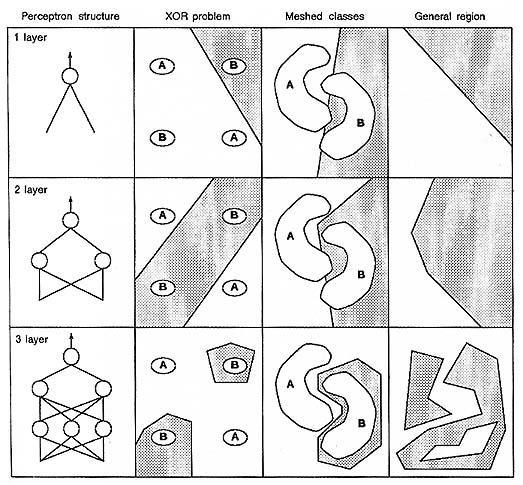
\includegraphics[width=10cm]{images/layers}
	\caption{Confronto tra architetture di rete.}
	\label{fig:architetture}
\end{figure}

\noindent Le potenzialità dei percettroni multistrato sono note da tempo, ma gli algoritmi per l'apprendimento sono stati ideati solo recentemente (1986).

\section{Previsione di serie temporali}
\label{sec:previsione_di_serie_temporali}

Le reti neurali, oltre alla classificazione e altri problemi \emph{discreti}, sono in grado di affrontare problemi \emph{continui} come la \textbf{previsione di una serie temporale}.

Si consideri una sequenza $P$ di vettori che dipendono dal tempo $t$:
\begin{align*}
	P = \{\vec{x}(t_0), \vec{x}(t_1), \cdots, \vec{x}(t_{i - 1}), \vec{x}(t_i), \vec{x}(t_{i + 1}), \cdots\}
\end{align*}
Per ottenere una serie $\{\vec{x}[t]\}$ da un segnale continuo $\vec{x}(t)$ è necessario \textbf{campionare} il segnale in punti discreti. 

Partendo da un tempo $t$ e procedendo a ritroso, otteniamo la serie temporale $\{\vec{x}[t], \vec{x}[t-1], \dots\}$. Lo scopo dell'analisi è di stimare $x(t)$ a un tempo futuro
\begin{align*}
	\hat{\vec{x}}[t+s] = f(\vec{x}[t], \vec{x}[t-1], \dots)
\end{align*}
dove $s$ è noto come \textbf{orizzonte della previsione}. Si tratta di un problema di approssimazione di una funzione che può essere risolto utilizzando una rete neurale a due strati.

\begin{thm}[Teorema dell'approssimazione universale - G. Cybenko, 1989 \& K. Hornik, 1991]
	Una rete neurale multistrato feed-forward con un singolo strato nascosto, un percettrone, che contiene un numero finito di neuroni nascosti è un approssimatore universale di funzioni continue su sottoinsiemi compatti $\mathbb{R}^n$.
\end{thm}
